\documentclass[../../dissertation.tex]{subfiles}
\begin{document}
The continuous-time random walk model on a graph is a Markov process where
transitions have a fixed probability per unit time, $\gamma$, of moving to
adjacent vertices, firstly introduced by \cite{montrollweiss1965}. Consider a
graph $G$ with $N$ vertices and no self-loops, this walk can be defined by the
linear differential equation that describes the probability of jumping to a
connected vertex in any given time 
\begin{equation}
	\frac{dp_i(t)}{dt} = \gamma \sum_j L_{ij} p_j(t), \label{eq:classicalContWalk}
\end{equation}
where $L$ is the Laplacian defined as $L = A - D$, and $p_j(t)$ is the time
dependent probability associated with each vertex transition. $A$ is the
adjacency matrix that represents each vertex connection, given by
\begin{equation}
	A_{ij} = \begin{cases} 1, & \mbox{if } (i,j)\in G \\ 0, & \mbox{otherwise,} \end{cases}
\end{equation}
and D is the diagonal matrix $D_{jj} = deg(j)$ corresponding to the
degree\footnote{The degree of a vertex refers to the number of edges that it is
connected to.} of vertex $j$.\par 

In the continuous-time quantum walk model (CTQW), the vertices are quantum
states that form the basis for the Hilbert space. The continuous-time quantum
walk model will also be described by a differential equation, the Schrödinger
equation
\begin{equation}
	i\hbar \frac{d\ket{\psi(t)}}{dt} = H \ket{\psi(t)}, \label{shrodinger}
\end{equation}
where $H = -\gamma L$ is the Hamiltonian of the system. More explicitly,
\begin{equation}
	H_{ij} = \begin{cases} 
		deg(j)\gamma, & \mbox{if } i= j; \\ 
		-\gamma, & \mbox{if } i\neq j\mbox{ and adjacent};\\
		0, & \mbox{if } i\neq j\mbox{ and not adjacent}.
	\end{cases}.
	\label{Hamilt}
\end{equation}\par

A general state of a system $\ket{\psi(t)}$ can be written as a function of
its complex amplitudes 
\begin{equation}
	q_i = \braket{i|\psi(t)},
\end{equation}
which means equation \eqref{shrodinger} can be rewritten as 
\begin{equation}
	i\hbar \frac{dq_i(t)}{dt} = \sum_j H_{ij} q_j(t).
	\label{eq:contWalkShrod}
\end{equation}
Comparing equations \eqref{eq:contWalkShrod} and \eqref{eq:classicalContWalk},
the Laplacian is replaced by the Hamiltonian, and the probabilities by
amplitudes. One of the main differences is the complex phase $i$, which will
result in a very different behavior.  Setting $\hbar = 1$ and solving the
differential equation results in the evolution operator of this walk 
\begin{equation}
	U(t) = e^{-iHt} = e^{i(\gamma L)t} = e^{i\gamma(A-D)t},
\end{equation}
In the regular graph case, where $D$ is simply the degree of the graph
multiplied by the identity matrix, $A$ and $D$ will commute, meaning that the
evolution operator can be written in terms of the adjacency matrix 
\begin{equation}
	U(t) = e^{i\gamma A t - i\gamma D t} = e^{i\gamma A t} e^{-i\gamma D t} = \phi(t) e^{i\gamma A t},
	\label{eq:contSimulUniOp}
\end{equation}
since the degree matrix becomes a global phase.  Applying this operator to an
initial condition $\psi(0)$, will give the state of the system at a time $t$
\begin{equation}
	\ket{\psi(t)} = U(t)\ket{\psi(0)}.
\end{equation}\par
\begin{figure}[!h]
	\centering
	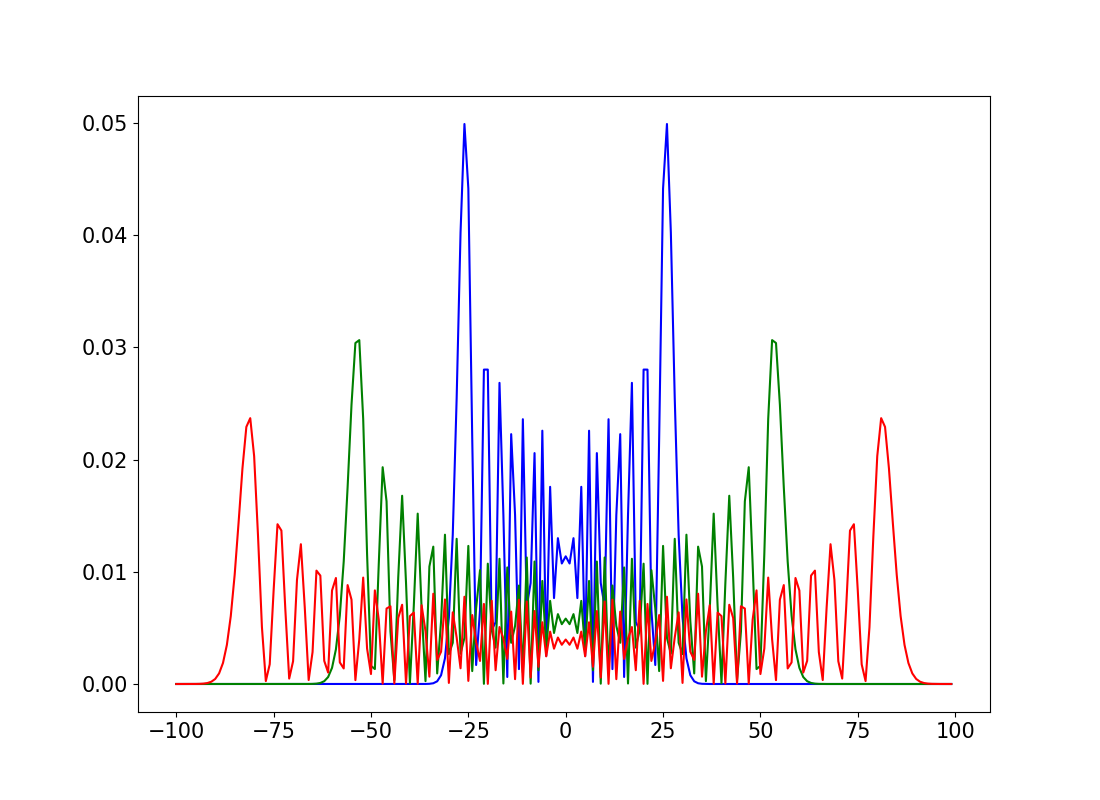
\includegraphics[scale=0.40]{img/ContQuantumWalk/ctqwMultipleTime.png}
	\caption{Probability distribution for the continuous-time quantum walk on a line, at $t=40$, $80$ and $120$, with initial condition $\ket{\psi(0)}=\ket{0}$ and $\gamma=\frac{1}{2\sqrt{2}}$.} 
	\label{fig:contdist0}
\end{figure}
Considering a uni-dimensional quantum system, each vertex will have at most 2
other neighboring vertices, reducing equation \eqref{Hamilt} to
\begin{equation}
	H_{ij} = \begin{cases} 
		2\gamma, & \mbox{if } i= j; \\ 
		-\gamma, & \mbox{if } i\neq j\mbox{ and adjacent};\\
		0, & \mbox{if } i\neq j\mbox{ and not adjacent}.
	\end{cases}
\end{equation}\par

For a more detailed visualization, this quantum walk model was coded in Python
and figure \ref{fig:contdist0} was obtained setting the transition rate to
$\gamma=\frac{1}{2\sqrt{2}}$ and the initial condition to $\ket{\psi(0)} = \ket{0}$.
A brief look at figure \ref{fig:contdist0} reveals several similarities to
previous models. The property of having two peaks away from the origin and low
probability near the origin is present across all the quantum walks. However, in
the continuous case, a symmetric initial condition is not needed. In the
staggered quantum walk model, the propagation of the walk could be altered by
changing the values of $\theta$, whereas in this case different values of
$\gamma$ and time will influence the probability distribution.\par
%TODO:\textcolor{red}{você pode dizer que o desvio padrão é proporcional ao $\gamma$ também}

Altering the initial condition will also differ in the
continuous-time example. For example, setting the initial condition to the
balanced superposition of states $\ket{0}$ and $\ket{1}$ has no effect on the
overall pattern of the probability distribution as seen in figure
\ref{fig:contdist2}. Both peaks are still present and at the same
distance from the origin, with intermediate amplitudes being attenuated
relative to figure \ref{fig:contdist0}. This behavior is in contrast with the previous
discrete-time cases, where a change in the initial condition would dictate the
number of peaks and where they would appear.
\begin{figure}[!h]
	\centering
	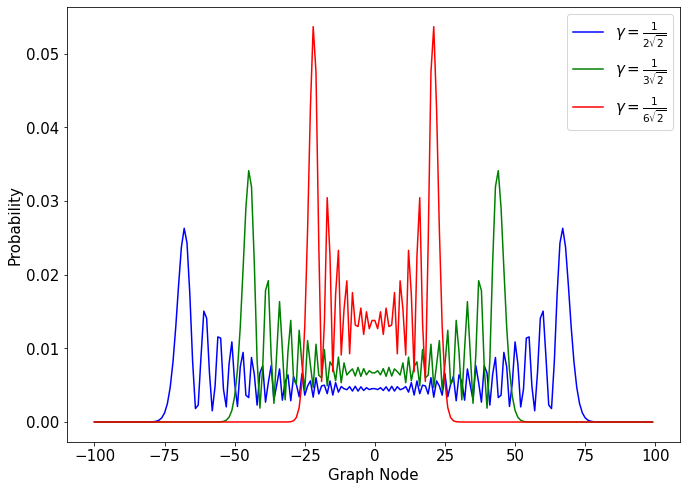
\includegraphics[scale=0.40]{img/ContQuantumWalk/ctqwMultipleGammaSup.png}
	\caption{Probability distribution for the continuous-time quantum walk on a line, at $t=100$, with initial condition $\ket{\psi(0)}=\frac{\ket{0}+\ket{1}}{\sqrt{2}}$, for multiple values of $\gamma$.} 
	\label{fig:contdist2}
\end{figure}
Figure \ref{fig:contdist2} also shows the influence of the transition rate
$\gamma$. As would be expected from equation \eqref{eq:contSimulUniOp}, the
effects are very similar to altering time, since both parameters are
multiplying in the exponential.\par

In conclusion, the purpose of this chapter was to present an overview of
several different models of a quantum walk. The probability distributions are
very distinct from the classical case, but relatively similar to each other.
The bigger differences between the models come from the size of the associated
Hilbert space. The staggered and continuous-time quantum walks have
Hilbert spaces equal to the space of the walker, whereas the coined
quantum walk also requires a space for the coin. It might seem unimportant now,
but it will play a major role when these models are translated into circuits,
since the size of the Hilbert space will have a direct relation with the number
of qubits required to perform the walk, which is a scarce resource for
\textit{Noisy intermediate-scale quantum} (NISQ) computers. Considering the
case of the coined quantum walk on a simple line graph, only one extra qubit
will be needed. However, as will be seen in the next chapter, the search problem is
optimal when performed over a complete graph which, in the coined case, will
double the number of required qubits. 

\end{document}
